\documentclass[a4paper,11pt]{article}
\usepackage{graphicx}
\usepackage[utf8]{inputenc}
\usepackage{hyperref}
\usepackage{placeins}
\usepackage[newfloat]{minted}
\usepackage{caption}

\newenvironment{code}{\captionsetup{type=listing}}{}
\SetupFloatingEnvironment{listing}{name=Code Overview}


\hypersetup{
    colorlinks=true,
    linkcolor=blue,
    filecolor=black,      
    urlcolor=blue,
    citecolor=black,
}
\begin{document}

\title{
    \textbf{Ques Report.}
}
\author{Adrian Jonsson Sjödin}
\date{Fall 2022}

\maketitle

\section{Introduction}


\section{Task}
Implement two different FIFO queues. One utilizing arrays and one utilizing a linked list structure.

For the linked list queue, first implement a linked list queue structure that only has one property,
the \textit{head}, and new elements are simply added to the end of this list. What are the drawbacks
to this implementation? What are the cost of removing the next element and adding a new element?

Change the linked list queue so that it holds a pointer to to the first element of the queue
(the \textit{head}), but also a pointer to the last element of the queue. This should allow one
to add a new node at the end directly without first having to traverse the list to find the last
node.

Now use the linked list queue to create a new iterator for the binary tree from last weeks assignment
that traverses the tree breath first.

The array implementation of the queue  should be dynamic and be able to increase in size, but also
optionally shrink in size.
\section{Method \& Theory}
A queue is a data structure that is built on the FIFO principle of \textit{first} element \textit{in} is \textit{first}
element \textit{out}. This structure is useful in real world application such as printers where we want to print a document but
at the same time send more documents to it to be printed after, in the order we sent them.
\subsection{Linked List Queue Without Second Pointer}

The first queue to be implemented was the linked list queue that did not have a pointer to the last element in the queue. The task
said to have a pointer to the head and add all new elements to the end of the list. I however went with the opposite and made the \textit{head}
pointer point to the last added element and that element in turn point to the old head. This way I can create a linked list that looks like in
figure \ref{fig:queueNoLast}. This shouldn't make a difference in the overall time it takes to add and remove elements to the queue. The way the task wanted
us to do would mean a cost of $\mathcal{O}(n)$, there $n$ is the size of the queue, for adding and $\mathcal{O}(1)$ for removing. My implementation would
simply reverse these costs.
\begin{figure}[h!]
    \centering
    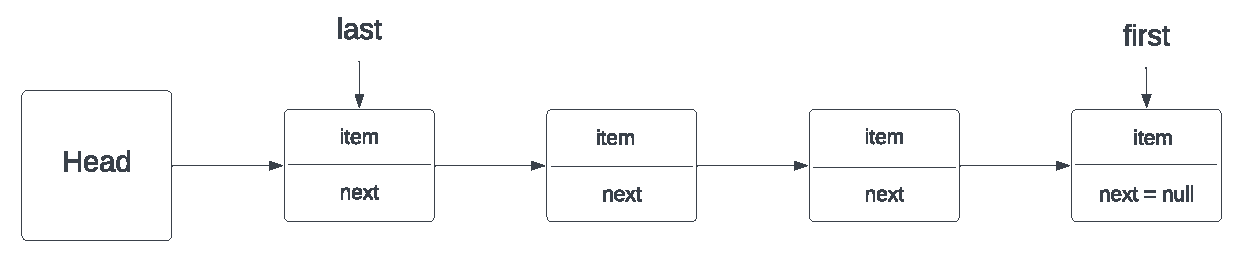
\includegraphics[width=.9\textwidth]{queue-no-last.pdf}
    \caption{Linked List Queue with only one pointer}
    \label{fig:queueNoLast}
\end{figure}

Adding an element to this queue is then just this one line of code {\tt this.queue = new Node(item, this.queue);}, in which we set the \textit{head} (here
called {\tt queue}) to be the new node and let that node point to the old \textit{head}, which depending on if the queue is empty or not before the add operation,
will have a pointer to an even older \textit{head}.

Removing elements from the queue is a bit more code but still quite straightforward. We first need to see if the queue is empty or not, but assuming that it is not
we then need to traverse the whole queue till we reach the element with a null pointer. This will be the first element added to the queue. Having found it we can
simply make the pointer for the previous element point to null instead and then return the found first element.

The code for {\tt add()} and {\tt remove()} can be seen in code overview \ref{code:queueNoLast}.

\subsection{Linked List Queue With Pointer To First \& Last Element}
The second linked list queue is an improvement over the the first one in that it has two pointers. One to the first element in the queue and one to the last.
This should allow us to make enqueue and dequeue operations at at constant time since we can directly add the new node to the end of the list without first having
to go through the whole list and find the last element, and we can also immediately retrieve the first element of the list.

The queue itself is a built up as depicted in figure \ref{fig:queue}. So when we initialize the queue with the constructor we first set {\tt first} and {\tt last}
to null. This way we now have an empty queue. We can then add elements to the queue using the {\tt enqueue} method. When adding elements we first need to check if
the queue is empty or not. That is done by looking at what {\tt first} is pointing at. If it is null the queue is empty and we can simply create a new node and let
both {\tt first} and {\tt last} point to that node. If {\tt first} is not null then we have something in the queue and {\tt first} and {\tt last} is already pointing
at something. We then create a new node and set {\tt last.next} to point at the new node to make sure every element in the queue is linked to the next element. We
then finally set {\tt last} to also point to the new node.
\begin{figure}[h!]
    \centering
    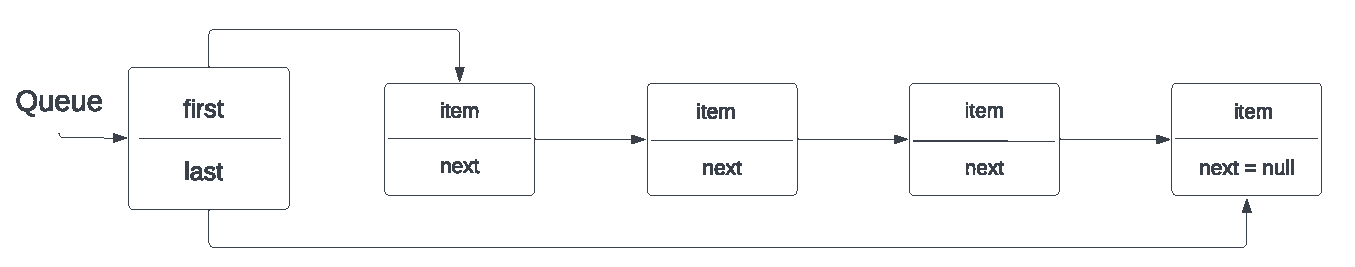
\includegraphics[width=\textwidth]{queue.pdf}
    \caption{Linked List Queue with two pointers}
    \label{fig:queue}
\end{figure}

The {\tt dequeue} method is quite similar in that we first check to see if the queue is empty or not. If it is we print a message telling us that and return null.
However if it is not empty then we start by retrieving the first element's item, then set {\tt first} to point at {\tt first.next} instead. We also need to check to
make sure that the retrieved element wasn't also the only element in the queue. This is done by checking wether or not the retrieve element is the same element as
the one {\tt last} is pointing at. If it was we also put {\tt last} to be null ({\tt first} would already have been set to null in the previous step in this case)
before returning the first element's item.

The code for {\tt enqueue()} and {\tt dequeue()} can be seen in code overview \ref{code:queue}.

\subsection{Breath First Traversal of Binary Tree}
Implementing a iterator for the binary tree created in last week's assignment required just some slight modifications to the stack iterator we created.
First instead of creating a stack in the {\tt TreeIterator} we create our queue that can accept nodes. In the constructor we then initialize the queue and
add the {\tt root} of the binary tree to the queue using {\tt enqueue()}.

The {\tt hasNext} method is left the same but calling the queue's {\tt isEmpty} method instead.

The {\tt next} method had to be completely altered. We still check wether or not we have a next node in the tree using the {\tt hasNext} method, but
then assuming we have one we pop the queue and set it as the current node. We then first check if current has a pointer down left and if it has we push that to
the queue. Then we check if it has a pointer down right and also push that to the queue if there is one. After this we simply return the value of the current node.

This way next time {\tt next} is called the node that was down left will be popped and set as current, and if that was null then it will not have been added and
instead the node down right will be the node popped. This will make it so that we traverse the binary tree from left to right, top to bottom, i.e. breath first
traversal.

The code for {\tt next} can be seen in code overview \ref{code:iterator}.
\subsection{Dynamic Queue Using Arrays}
Lastly we were supposed to implement a queue using arrays. This was by far the trickiest thing to implement since
we needed to keep track of where in the array we where storing the elements.

The idea is that we create an empty array of a fixed size that can hold generic objects, and where each element is
initially set to null. We can then add elements to the que by placing them in the array. To keep track of where the first
element and the last element is located in the array we also need two pointers, {\tt first} and {\tt last}. These are
simply storing the index of the array where the first and last element in the queue is stored.

When adding an element to the queue there is a lot of things to consider. Here I am going to go through them one after
the other in the order that I implemented them in the {\tt enqueue} method.

\subsubsection{{\tt enqueue(Item item)}}
First we need to check if the array is empty. This is done by having a private field {\tt itemsInQueue} which tracks
how many elements we have added to the queue. If the queue is empty we store the element at the index value given
by {\tt first} ({\tt first} and {\tt last} are set to 0 when queue is first created), and then increment {\tt last}
and {\tt itemsInQueue} by one. This will make it so that {\tt last} points to the next empty spot in the array.

If it is not empty then we do one or two things out of four things. First we check if {\tt last -1 == size -1}
(meaning is the last index in the array taken) and check if the array is not full. If this gives {\tt true} then it
means that we have dequeued elements at the front of the array and that there's free space we can use. We then set
    {\tt last = 0} which will allow us to reuse that space. After this check we also check if the array is full and
if it is we resize it. This will not happen in this case since we said the earlier check gave {\tt true}. After
this check we have yet another check and this one checks wether or not {\tt last == 0}. This is to see if we should
add the new element to the start of the array and reuse space or not. If it gives false we simply add it at the
index value of {\tt last} and then increment it and {\tt itemsInQueue} with one.  If it gives {\tt true}, which it will
in this case we do the same thing but the index value of {\tt last} will now be $0$.

As mentioned this was quite tricky and also hard to describe in text. To get a better overview of how this works I've
included the code for this method in code overview \ref{code:arrayAdd}.

\subsubsection{{\tt dequeue()}}
The {\tt dequeue} method in comparison is quite simple. Here we first check if the queue is empty and if it is we inform
the user and return null. If it is not we do basically the same operation as in {\tt dequeue} for the linked list. We
start with retrieving the first item from the array by retrieving the element at the index value of {\tt first} in
the array. We then set that spot to null and increment {\tt first} by one and decrement {\tt itemsInQueue} by one.
After this we check if {\tt itemsInQueue <= size / 4}. If this gives {\tt true} that means we have a lot of empty space
in the array and we want to shrink it. To do this we call {\tt resize()} which will shrink the array. Now lastly we
return the retrieved item.

\subsection{{\tt resize()}}
The {\tt resize} method is what makes this queue dynamic. It will expand it if it is full and shrink it if there's
a lot of empty space

\section{Discussion}


\newpage
\FloatBarrier
\section*{Code}
All the code can be found here: \href{https://github.com/adrian-jonsson-sjoedin/ID1021-AlgoData/tree/main/Tasks/Trees/src}{GitHub}

\begin{code}
    \captionof{listing}{Add and remove in first linked list queue}
    \label{code:queueNoLast}
    \begin{minted}{java}
public void add(Integer item) {
    this.queue = new Node(item, this.queue);
}
public Integer retrieve() {
    Node prev = null;
    Node current = this.queue;
    if (isEmpty()) {
        System.out.println("queue is empty");
        return null;
    }
    while (current.next != null) {
        prev = current;
        current = current.next;
    }
    this.queue = prev;
    return current.item;
}
\end{minted}
\end{code}

\begin{code}
    \captionof{listing}{Enqueue and dequeue in second linked list queue}
    \label{code:queue}
    \begin{minted}{java}
public void enqueue(Item item) {
    Node newNode = new Node(item, null);
    if (this.first == null)
        this.first = newNode;
    if (this.last != null)
        this.last.next = newNode;
    this.last = newNode;
}
public Item dequeue() {
    if (this.first == null) {
        System.out.println("dequeue(): queue is empty");
        return null;
    }
    Item returnedItem = this.first.item;
    Node retrievedNode = this.first;
    this.first = this.first.next;
    if (retrievedNode == this.last)
        this.last = null;
    return returnedItem;
}
\end{minted}
\end{code}

\begin{code}
    \captionof{listing}{The {\tt next()} method for the iterator}
    \label{code:iterator}
    \begin{minted}{java}
public Integer next() {
    if (!hasNext()) {
        throw new NoSuchElementException();
    }
    Node current = queue.dequeue();
    if (current.left != null)
        queue.enqueue(current.left);
    if (current.right != null)
        queue.enqueue(current.right);
    return current.value;
}
\end{minted}
\end{code}

\begin{code}
    \captionof{listing}{Array implementation of {\tt enqueue(Item item)}}
    \label{code:arrayAdd}
    \begin{minted}{java}
public void enqueue(Item item) {
    if (isEmpty()) {
        this.queue[this.first] = item;
        this.itemsInQueue++;
        this.last++;
        return;
    }
    if (!isEmpty()) {
        if ((this.last - 1) == (this.size - 1) && !isFull()) {
            this.last = 0;
        }
        if (isFull()) {
            resize();
        }
        if (this.last == 0) {
            this.queue[this.last] = item;
            this.last++;
            this.itemsInQueue++;
        } else {
            this.queue[this.last] = item;
            this.last++;
            this.itemsInQueue++;
        }
    }
}
\end{minted}
\end{code}

\begin{code}
    \captionof{listing}{Array implementation of {\tt dequeue()}}
    \label{code:arrarDequeue}
    \begin{minted}{java}
public Item dequeue() {
    if (isEmpty()) {
        System.out.println("dequeue(): queue is empty");
        return null;
    }
    Item returnedItem = this.queue[this.first];
    this.queue[this.first] = null;
    this.first++;
    this.itemsInQueue--;
    if (this.itemsInQueue <= (this.size / 4)) {
        resize();
    }
    return returnedItem;
}
\end{minted}
\end{code}

\begin{code}
    \captionof{listing}{Array implementation of {\tt dequeue()}}
    \label{code:arrayDequeue}
    \begin{minted}{java}
public void resize() {
    int newSize;
    int j;
    Item[] newQueue;
    if (isFull()) {
        newSize = this.size * 2;
        newQueue = (Item[]) new Object[newSize];
        j = 0;
        for (int i = this.first; i < this.size; i++) {
            newQueue[j] = this.queue[i];
            j++;
        }
        for (int i = 0; i < this.first; i++) {
            newQueue[j] = this.queue[i];
            j++;
        }
    } else {
        newSize = this.size / 2;
        newQueue = (Item[]) new Object[newSize];
        j = 0;
        for (int i = this.first; i < this.size; i++) {
            if (this.queue[i] == null)
                break;
            newQueue[j] = this.queue[i];
            j++;
        }
        if (this.last < this.first) {
            for (int i = 0; i < this.last; i++) {
                newQueue[j] = this.queue[i];
                j++;
            }
        }
    }
    this.queue = newQueue;
    this.size = newSize;
    this.first = 0;
    this.last = j;
    newQueue = null;
}
\end{minted}
\end{code}
\end{document}
